\chapter{Угадыватель чисел}
\label{ch:guessnumbers}

\section{Описание задачи}

\newthought{ Суть предлагаемой нами задачи} описана в старинной книге автора первого в России учебного пособия по математике, Л. Ф. Магницкого, "Арифметика", в главе: "Об утешных некиих действиях, через арифметику употребляемых".

Для начала предложим игроку загадать число, равное номеру любого дня недели. Дни недели пронумеруем от 1 (понедельник) до 7 (воскресенье). Далее попросим загадавшего выполнить следующие действия:

\begin{enumerate}
\item Умножить номер загаданного дня недели на 2..
\item К полученному произведению необходимо прибавить 5.
\item Затем полученную сумму умножить на 5.
\item Полученное число умножить на 10.
\item Назвать результат вычислений.
\end{enumerate}

Таким образом, мы легко сможем определить какое число загадал игрок.

\section{Решение задачи}
Раскроем секрет математического фокуса.
Чтобы перейти от полученного числа к загаданному числу, необходимо вычесть из него 250. Таким образом, мы получим число, в котором номер дня недели – число сотен. Рассмотрим доказательство решения задачи. Пусть {a} — искомое число (день недели). Выполним указанные действия над числом {a}:
\begin{enumerate}
   \item 2\cdota = 2a

   \item 2\cdota+5 = 2a + 5

   \item 5\cdot(2\cdota+5) = 10a + 25
 
   \item (10a+25)\cdot 10 = 100a + 250
 
   \item 100a+250 — 250 = 100a
\end{enumerate}

Таким образом, мы получим число, в котором номер дня недели – число сотен ({{a}})

\section{Реализвция приложения}

В данной программе загаданный игроком номер дня недели это то, что мы будем вычислять.

Создадим глобальную переменную number для хранения числа, загаданного игроком. Изначально присвоим переменной значение 0, а так как ноль не является допустимым загадываемым числом, переменная не будет хранить в себе число, которое мог бы загадать пользователь.

\subsection{Процедура selectVisibleImage}

Процедура selectVisibleImage (см. рисунок ~\ref{fig:block:click:select:visible:image}) определяет какое изображение с числом необходимо показать игроку. В случае, если число не было определено показывается изображение с вопросительным знаком (Image8) Сообщение "Пожалуйста, введите полученное число." (ErrorLabel) становится видимым, если ничего не было введено пользователем и он нажал на кнопку "Узнать ответ".
\begin{figure}
    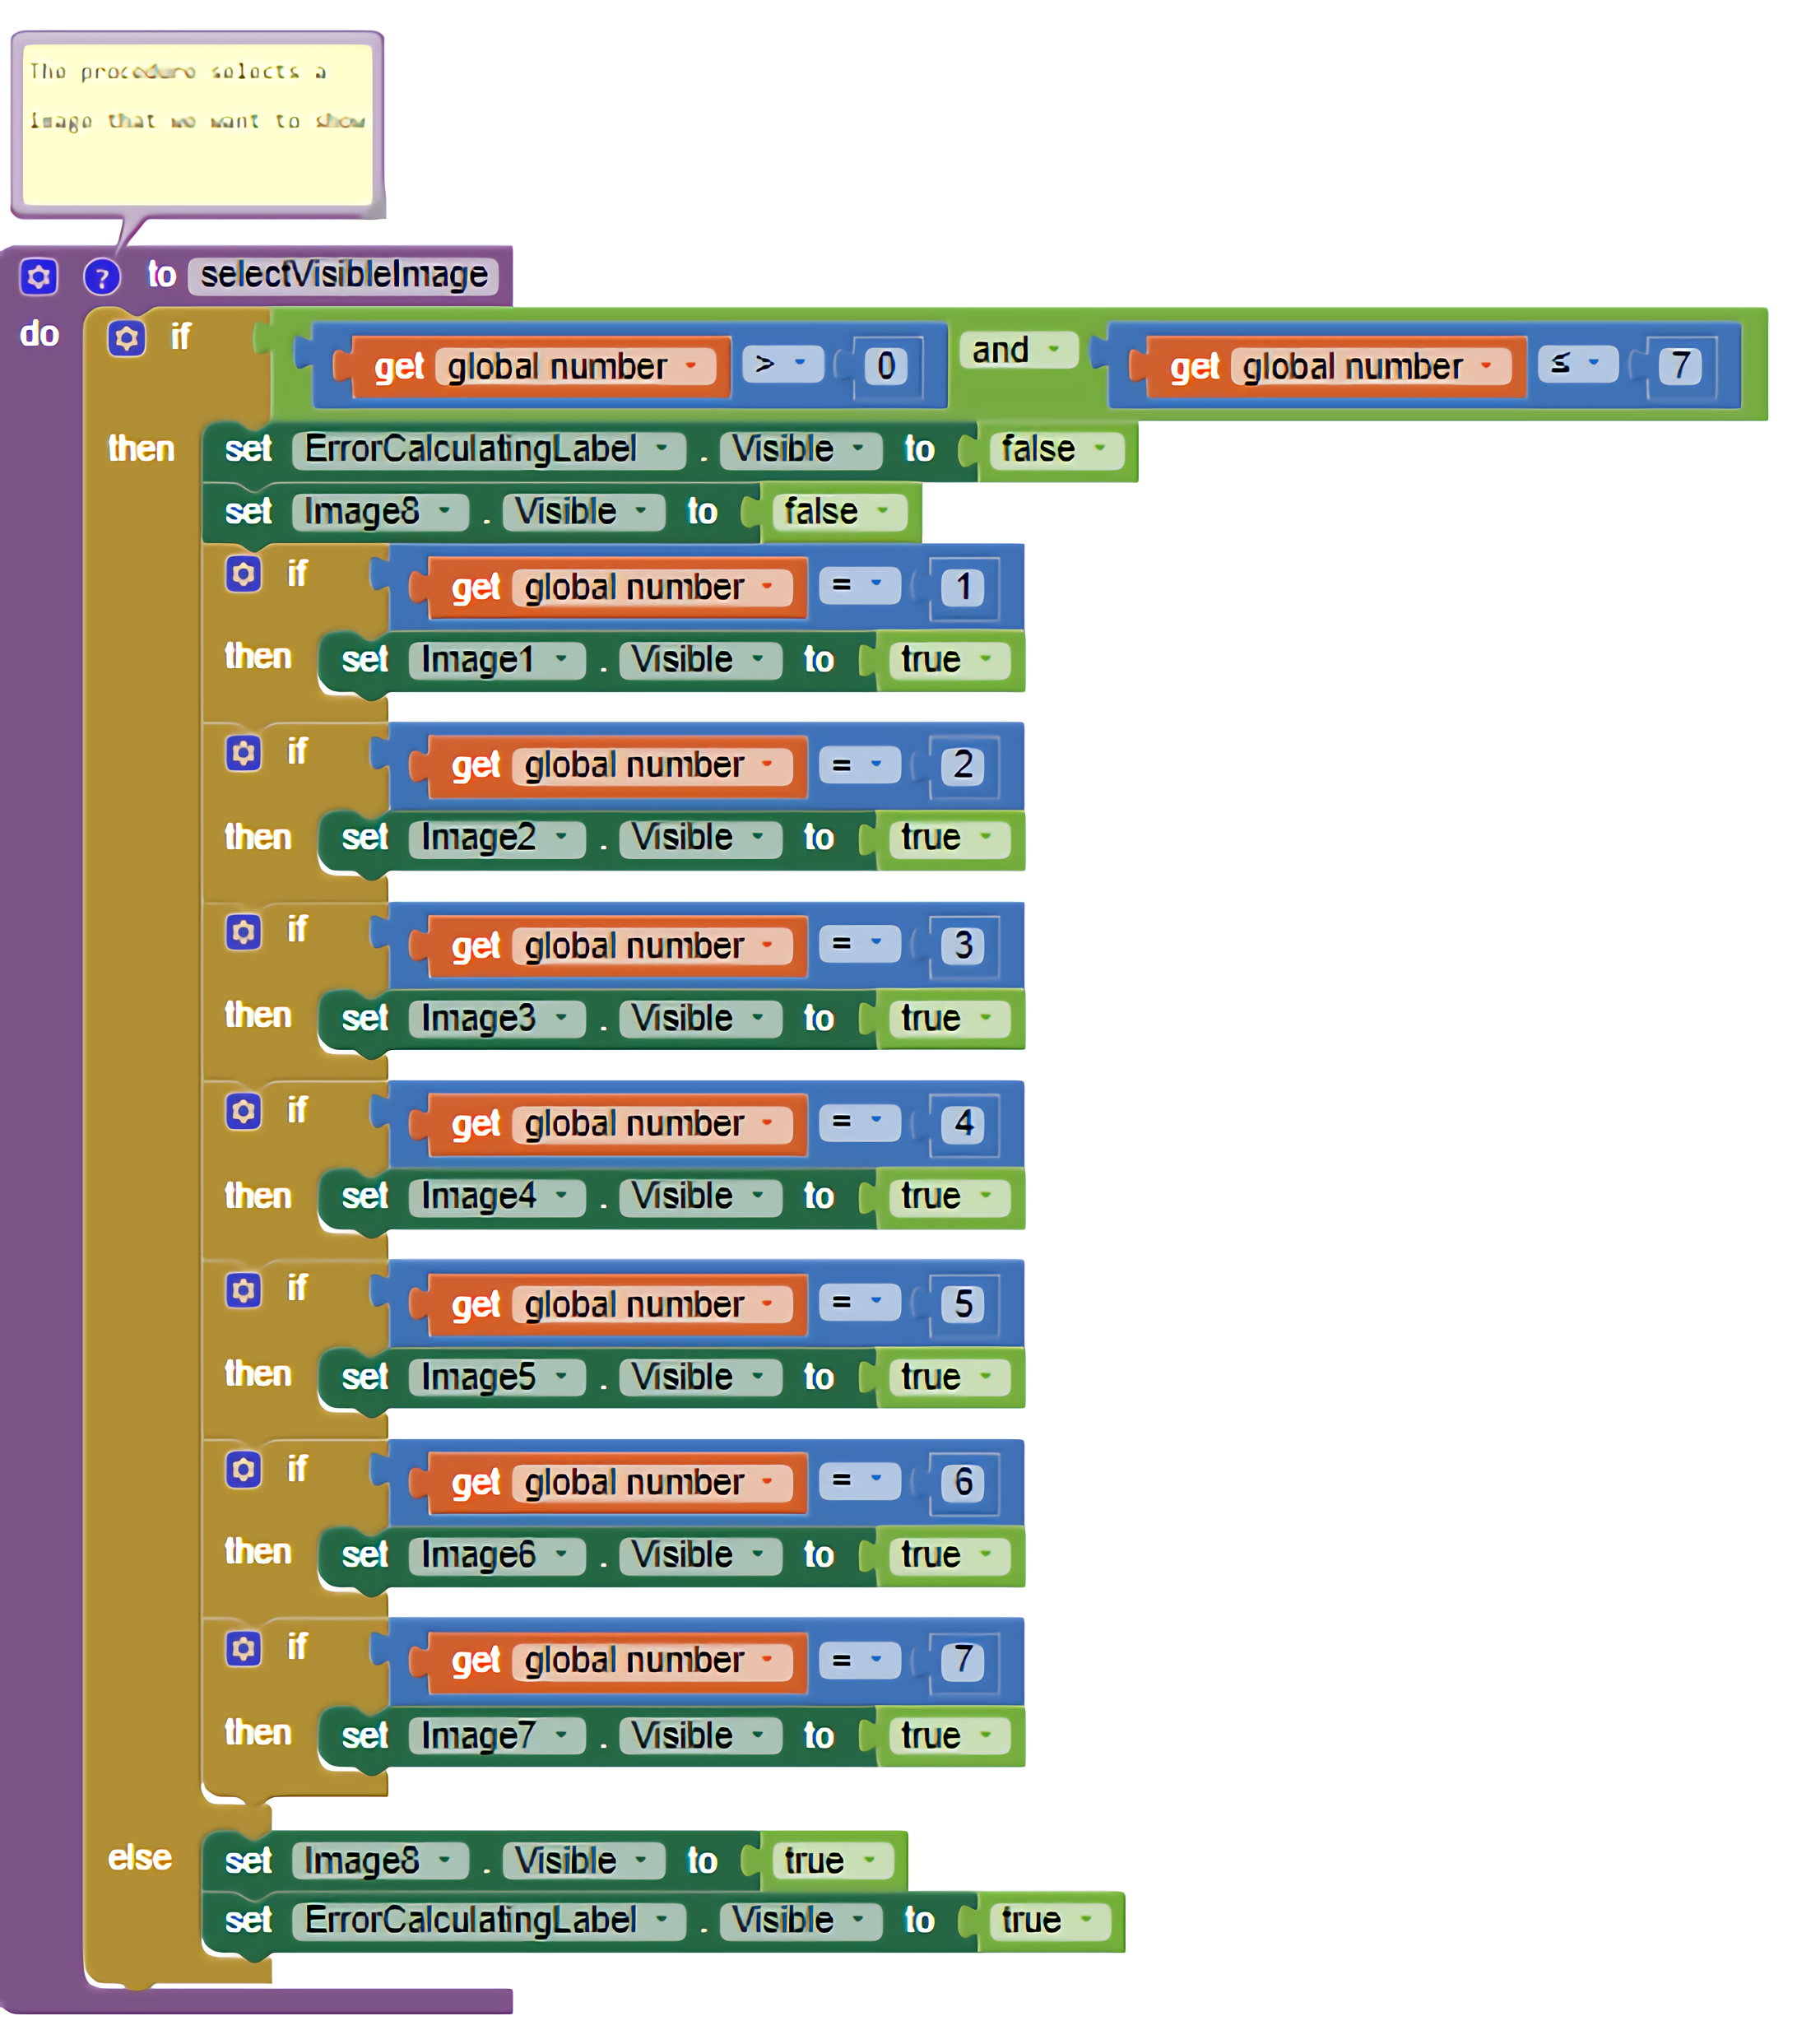
\includegraphics{./graphics/programs/guess_numbers/procedure_selectVisibleImage_AppInventor_2018.png}
      \caption[Процедура selectVisibleImage.][6pt]{Процедура selectVisibleImage управляет отображением изображений с цифрами.}
    \label{fig:block:click:select:visible:image}
  \end{figure}
Рассмотрим пример. Допустим, игрок загадал число 3. Приложение на основании введенного пользователем числа в поле numberText (в данном случае должно быть 550) на экране FinalScreen, считает и записывает новое значение переменной number, равное трем. Процедура же ставит в соответствие значению переменной number изображение с определенным числом и показывает его пользователю, например, изображение числа 3 (Image3). Если переменная number содержит в себе значение не в интервале от 1 до 7, то будет показано изображение со знаком вопроса (Image8) и текст надписи ErrorСalculating станет видимым.

Важно отметить, что перед выполнением условий сравнения переменной number с числом, выполняется установка свойства Видимый (Visible) в false у элементов Image8 и ErrorСalculating. Тем самым мы отмечаем, что пока ошибок в вычислениях не произошло и заранее убираем с экрана знак вопроса.

\subsection{Работа с экранами}
При проектировании приложения были учтены рекомендации из официальной документации App Inventor по ограничению количества экранов во избежание проблем с переполнением памяти.

Поэтому в игре используется четыре экрана (рекомендуемое количество < 10):
\begin{enumerate}
\item Screen1 — главный экран приложения представляющий из себя меню игры.
\item About — экран, содержащий основную информацию о приложении.
\item Steps — экран, который представляет собой описание последовательности действий, которые необходимо выполнить пользователю. На экране есть кнопки для переходов между описанием действий, изменяющих видимость элементов, тем самым визуально делается переход к определенному шагу.
\begin{enumerate}
  \item "На шаг назад" (previousStepButton) показывает описание предыдущего действия.
  \item "Далее" (nextStepButton) перемещает на шаг вперед.
  \item "В главное меню" (backToMainMenuButton) возвращает игрока на главный экран.
\end{enumerate}
\item FinalScreen — экран, на котором заканчивается игра. Здесь пользователю необходимо ввести получившееся в результате вычислений число и нажать кнопку "узнать ответ", чтобы приложение вывело на экран загаданное игроком число.

\end{enumerate}

\newthought{The front matter} of a book refers to all of the material that
comes before the main text.  The following table from shows a list of
material that appears in the front matter of \VDQI, \EI, \VE, and \BE
along with its page number.  Page numbers that appear in parentheses refer
to folios that do not have a printed page number (but they are still
counted in the page number sequence).
